%!TEX root = ../article.tex

% A new section
\section{Background}
\label{sec:background}
In order to develop a programming environment for \gls{gd} that works as a web application, we first need to study the currently available \gls{gd} environments.

Not all presented solutions are used exclusively for \gls{gd}.
\gls{gd} encompasses both 3D modeling and programming, so it makes sense to not only look at systems that explore both aspects, but also systems that explore just one of them.
Furthermore, the presented solutions include both desktop-based and web-based applications to allow the understanding of what is currently possible in the cloud and how it compares to what is available on the desktop.


\subsection{Related Work}
\subsubsection{LightTable}
\label{lighttable:related}
LightTable\cite{lighttable2015site} is a code editor for the Clojure programming language\cite{hickey2008clojure} and is an example of a desktop application that uses web technologies.

Although not related to \gls{gd}, LightTable proposed some interesting features and concepts for \glspl{ide}.
%Why is LightTable relevant?
One of these is the use of the drafting table as metaphor.%
\footnote{http://www.chris-granger.com/2012/04/12/light-table-a-new-ide-concept/ (last accessed on 10/05/2017)}
Instead of displaying the contents of entire files, LightTable divides the code into meaningful units and displays them as small editors spread over the table's surface.
Figure~\ref{fig:lt:draft:table} shows an example of this metaphor, which has some resemblance to node-based/visual programming environments, since the programmer still has to think of how to arrange what is on the table.

\begin{figure}
  \centering
  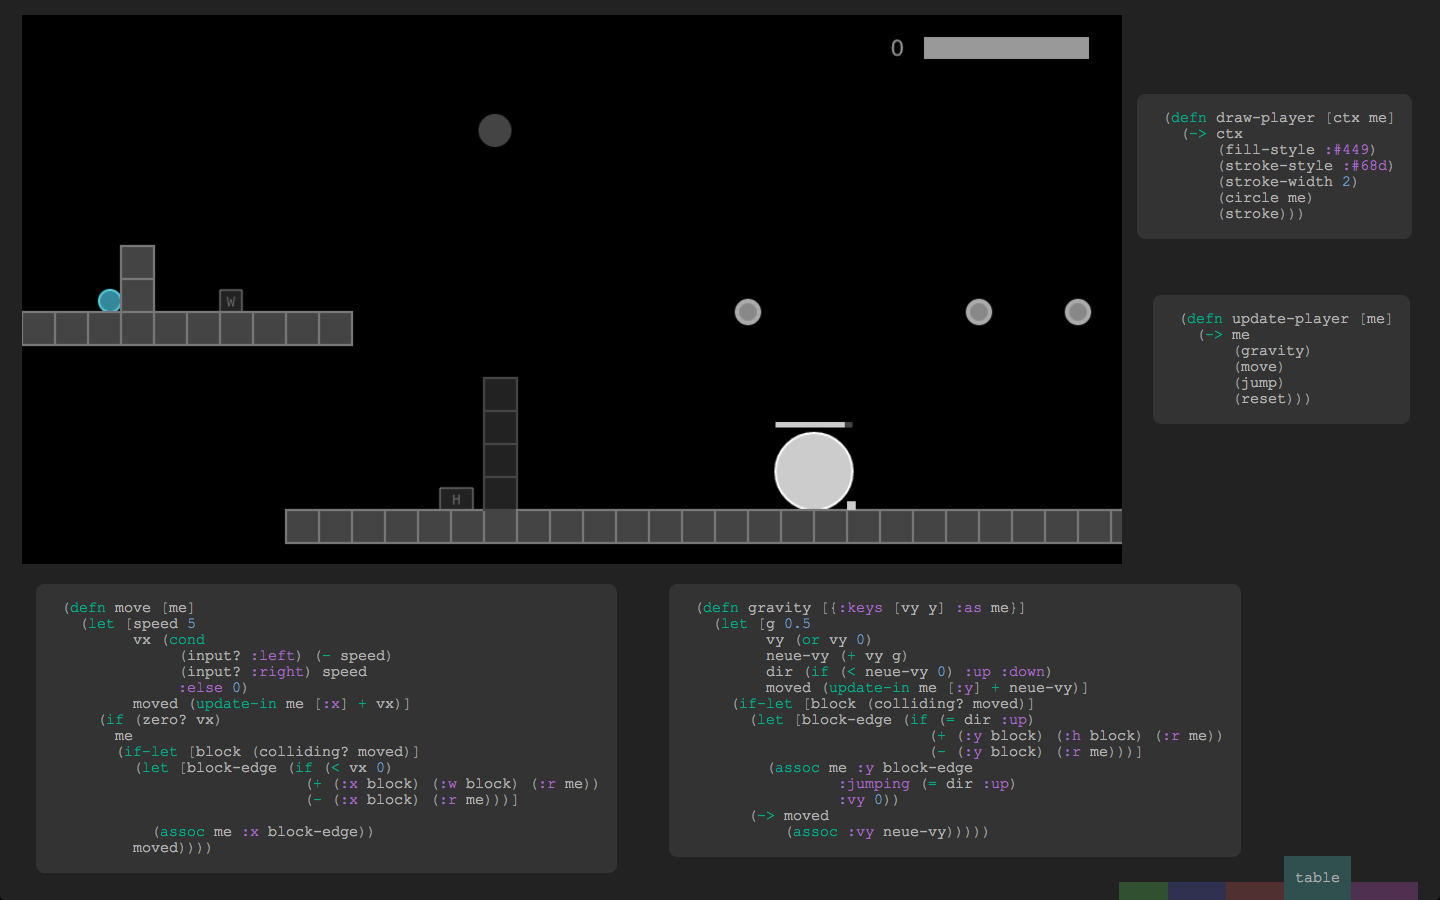
\includegraphics[width=1.0\linewidth]{./\figurePath/lt_game_example}
  \caption[LightTable's drafting table showing a game.]{LightTable's drafting table. A game is being run inside it while some of its code is displayed in separate editors.}
  \label{fig:lt:draft:table}
\end{figure}

%LightTable "function navigation"
Other feature deals with making navigation in Clojure code bases easier.
In Clojure, functions are defined inside namespaces and all Clojure definitions (like functions, variables, macros) are stored in text files.
Navigating among definitions and the namespace structure should not get in the way of editing code.
To make editing easier, LightTable provides a \emph{namespace browser} that allows to find functions and a \emph{code document} where functions can be added for editing, without moving them out of their namespace or displaying entire files where they are defined.

%LightTable "variable substitution"
Another interesting feature of LightTable is its ability to show data flow in a function call.
Since the main purpose of a function is to transform its input data into its output data, it helps to see what happens to the data on each step of the function.
To achieve this, LightTable overlays variable values and return values, respectively, on each variable occurrence and expression of the function.

This last feature has the problem of not being capable of showing the data-flow for more than one run of a part of the code.
If a function is called more than once, then it will be more useful to show the data-flow of all the calls.


\subsubsection{IPython}
\label{section:ipython:related}
IPython\cite{PER-GRA:2007} is a programming environment directed towards providing better, more straightforward, scientific computing.

%Why is it important? I cannot imagine designers using it.
IPython can be used as a command shell by using its notebook \gls{ui}, the IPython notebook.
As seen in Figure~\ref{fig:ipython:notebook}, IPython's notebooks can contain not only source code but also results and rich text.
These notebooks are displayed using an interactive web page.

The style of producing notebooks in IPython is one that mixes programming, writing and exploring.
Interestingly, this style is also part of a designer's processes.
Like a scientist, the designer also has to do exploration of ideas (design ideas in his case), reach conclusions (finished designs) and share his work with others (fellow designers, clients, friends, blog readers).
Unfortunately, although IPython notebooks are natural tools for exploration, they do not provide domain specific functionality for architecture.

%IPython architecture
To allow more flexibility between the core computing functionality and the \gls{ui}, IPython was decomposed into execution kernels, a communication protocol, and several front-ends.
Execution kernels are responsible for running the code of notebooks, and front-ends implement the \gls{ui}, as is the case of IPython's notebooks.
The communication protocol defines how communication between execution kernels and front-ends is done.
With this, it is possible to implement new execution kernels for running code from a programming language not yet implemented or an alternative front-end different from IPython notebooks.
Moreover, the communication protocol also allows execution kernels and front-ends to run on different computers\cite{PER-GRA:2007}.

\begin{figure}
	\centering
	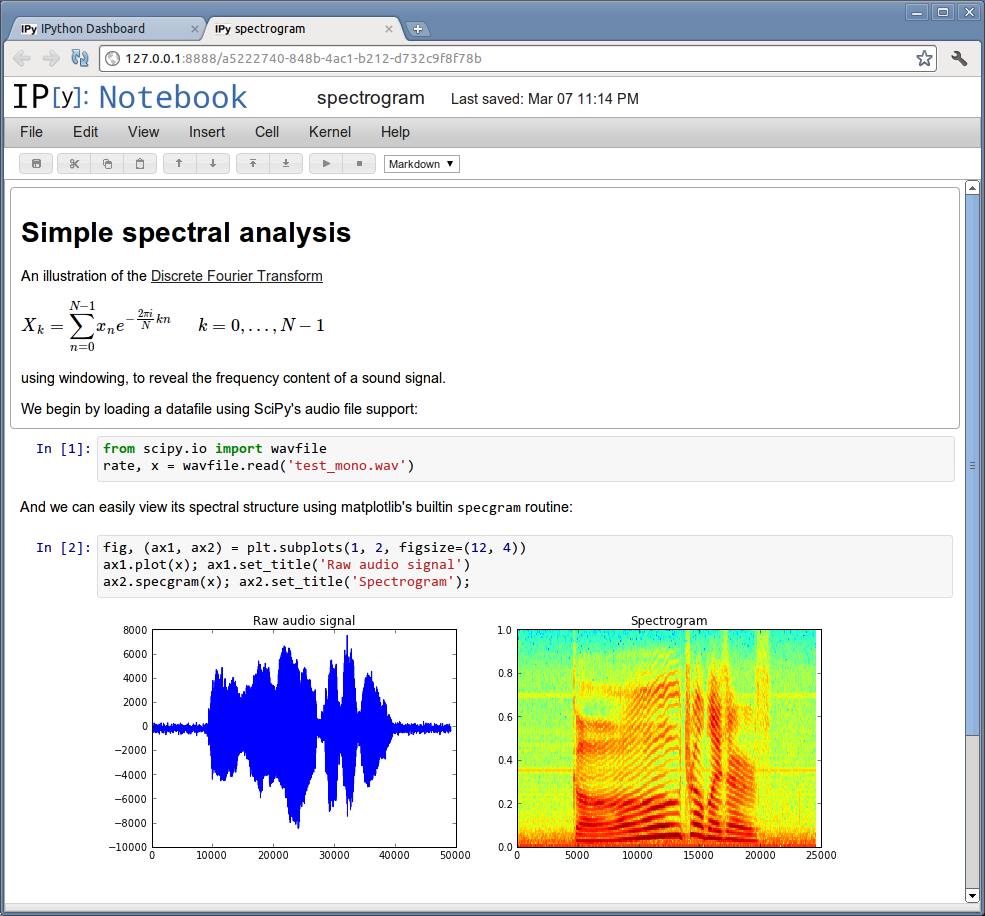
\includegraphics[width=1.0\linewidth]{\figurePath/ipython_notebook}
	\caption{An IPython notebook with rich text, mathematical notation, source code and results from executing such code.}
	\label{fig:ipython:notebook}
\end{figure}


\subsubsection{OpenJSCAD}
OpenJSCAD\footnote{\url{http://openjscad.org/} (last accessed 10/05/2017)} is a project aiming to implement OpenSCAD\footnote{\url{http://www.openscad.org/} (last accessed 10/05/2017)} using web technologies.
OpenJSCAD supports most of OpenSCAD's functionality.
Like OpenSCAD, it focuses on creating 3D models for 3D printing.
Similarly to the \gls{gd} approach, to actually model in OpenJSCAD, the user has to write a program in either JavaScript or OpenSCAD's language.

OpenJSCAD provides two user interfaces, one \acrfull{cli} and one \acrfull{gui}, the latter implemented as a web page.%
\footnote{https://github.com/Spiritdude/OpenJSCAD.org (last accessed on 10/05/2017)}
Moreover, the first can be used for batch processing, while the second integrates an editor to edit a program and a 3D view for viewing the corresponding results.
This separation enables the use of OpenJSCAD for programming, without requiring the programmer to install anything more than a web browser, which is almost always already installed.

OpenJSCAD makes its functionality available as functions, as well as methods on its objects, which makes writing programs more flexible.
Both functions and methods return new objects and do not have side-effects.
This allows the programmer to use the functional programming paradigm and makes it easier to understand programs, as there are less side-effects that could change their behavior.


\subsubsection{Processing}
\label{section:processing:related}
Processing\cite{reas2007processing} is a programming language and a development environment aimed at ``promoting software literacy in the visual arts and visual literacy within technology''.%
\footnote{Quoting https://www.processing.org, 9/Nov/2015.}

Processing enables everyone to write programs that both draw to the screen and react to input from the user, like moving the mouse or pressing a key on the keyboard.
It makes this possible by implementing most of the functionality that is commonly required, like initializing the drawing surface, so the programmer only has to implement the functionality specific to the result he wants to achieve.
The code in Listing~\ref{lst:simple:processing}, for instance, is what is needed to setup a drawing canvas, its background color, and continuously draw a line from the mouse position to a point on the canvas.

To use Processing's programming language, one needs to use its \gls{ide}, the \acrfull{pde}.
As shown in Figure~\ref{fig:proc:dev:env}, the \gls{pde} includes a text editor with syntax highlighting and runs Processing programs.

\begin{listing}
\begin{minted}[frame=lines]{java}
//Hello mouse.
void setup() {
   size(400, 400);
   stroke(255);
   background(192, 64, 0);
}

void draw() {
   line(150, 25, mouseX, mouseY);
}
\end{minted}
	\caption[A simple Processing sketch]{A simple Processing sketch}
	\label{lst:simple:processing}
\end{listing}

\begin{figure}
	\centering
	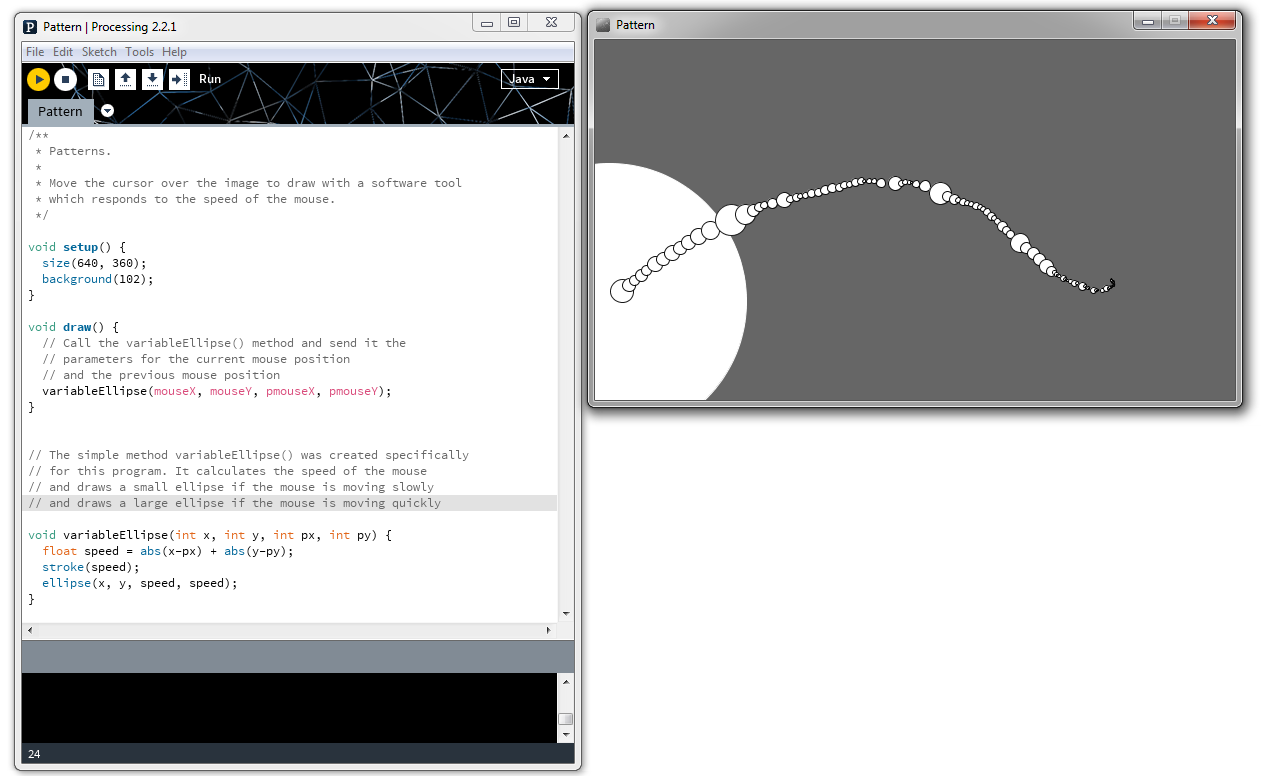
\includegraphics[width=1.0\linewidth]{\figurePath/proc_dev_env}
	\caption{On the left: The \gls{pde} displaying an example \emph{sketch} while it is being run. On the right: The drawing window to which the \emph{sketch's} instructions are applied.}
	\label{fig:proc:dev:env}
\end{figure}

Processing is sometimes used by architects for exploring design ideas.
However, since most of its functionality revolves around graphics for the visual arts, its use is normally restricted to 2D designs and cannot be used as a full-fledged tool for \gls{gd}.

Several projects have stemmed from Processing to extend its functionality to different programming languages.
These include Processing.py\footnote{http://py.processing.org/ (last accessed on 10/05/2017)}, that extends the \gls{pde} to support Python, and p5.js\footnote{http://p5js.org/ (last accessed on 10/05/2017)}, that provides JavaScript libraries to create interactive web pages.


\subsubsection{DesignScript}
\label{section:designscript:related}
DesignScript\cite{aish2012designscript} is a programming language that was designed to suit the needs of architecture related design.

%DesignScript programming paradigms
DesignScript uses concepts from multiple programming paradigms like object-oriented, functional, and associative programming\cite{aish2012designscript}.
Entities have properties that can be either data or functions, like in object-oriented languages; functions' most important role is to take some input and produce some output without producing side-effects, like in functional languages; and dependencies among variables are retained, like in associative languages.

%DesignScript primitives
Being a domain-specific language for architecture, DesignScript provides functions for 3D modeling, such as creating concrete 3D objects, like cubes and spheres, as well as abstract geometry, like planes and points, that is used as scaffolding.

DesignScript also supports lists of values and lets them be used in place of single parameters in calls to functions as it is common to start with one value and then scale up to many.
This lets architects use lists more easily, as they do not have to use loops to extract values and pass them to functions.

Having modeling primitives and combining several programming paradigms allows the architect to draw from knowledge about architecture modeling, while empowering him to express the processes in which those primitives are used.

DesignScript is used in several environments, all of which are desktop applications.
These include a textual editor in Autodesk AutoCAD, a dedicated graph editor called DesignScript Studio and Dynamo, which integrates with Autodesk Revit.
Both DesignScript Studio and Dynamo use graph based program editing.


\subsubsection{Rosetta}
\label{section:rosetta:related}
Rosetta\cite{de2012modern,lopes2011portable}, shown in Figure~\ref{fig:rosetta:ex}, is an environment for \gls{gd}.

Rosetta's motivation is to allow architects to write portable \gls{gd} programs that generate equivalent models in any \gls{cad} applications they use.
Rosetta allows architects to choose the front-end programming language and the back-end where the primitive operations will be performed\cite{de2012modern}.%
\footnote{Some front-ends supported by Rosetta are AutoLisp (one of AutoCAD's programming languages), Javascript, Racket and Python; some of the supported back-ends include CADs like Autodesk AutoCAD, Autodesk Revit, Sketchup, and Rhinoceros 3D and also graphics libraries like TikZ and OpenGL.}
With this, architects can experiment with \gls{gd} without having to switch \gls{cad}, and they can also share programs with others using different \glspl{cad}.

Additionally, Rosetta also allows programs written in one programming language to use not only parts from programs written in the same language, but also from programs written in other languages.
This makes it possible for architects to share programs written in different programming languages, and it also allows them to choose the programming language that best fits each part of the program they are working on.

\begin{figure}
	\centering
	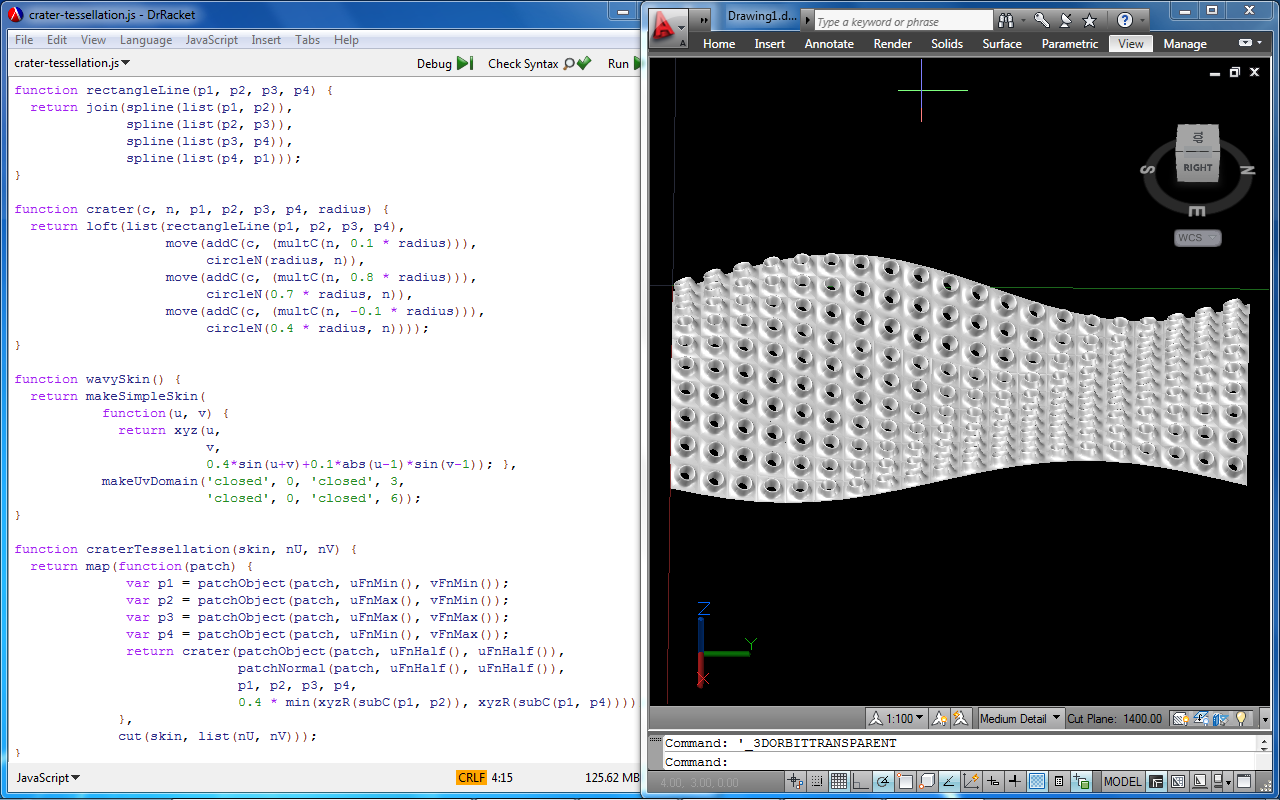
\includegraphics[width=1.0\linewidth]{\figurePath/rosetta_js_autocad}
	\caption{A Rosetta program (left) and AutoCAD displaying its results (right). The program is written in Javascript.}
	\label{fig:rosetta:ex}
\end{figure}


\subsubsection{OnShape}
OnShape\footnote{https://www.onshape.com/ (last accessed on 10/05/2017)} is a cloud-based \gls{cad} application that can be accessed using either a web browser or its mobile app.
As opposed to the systems we talked about earlier, OnShape is a \gls{cad} for mechanical modeling and, as such, its users are familiar with \glspl{cad} like SolidWorks\footnote{\url{http://www.solidworks.com/} (last accessed on 10/05/2017)} and Autodesk Inventor.%
\footnote{\url{http://www.autodesk.com/products/inventor/overview} (last accessed on 10/05/2017)}

OnShape has version control of project documents (drawings, 3D models, text documents) and supports real time collaboration.
Like most cloud applications, OnShape promotes collaboration on development teams where team members work remotely.
In order to do this, it allows users to work on the same copy of files, as opposed to each working with his own copy, and therefore changes are synchronized automatically.
As users can edit the same copy of a file at the same time, OnShape shows each user what the others are doing to enhance real time collaboration.

OnShape also includes a dedicated programming language, FeatureScript\footnote{https://www.onshape.com/featurescript (last accessed on 10/05/2017)}, for defining features for its models.
OnShape includes an \gls{ide} for FeatureScript, but the language does not aim to replace OnShape's modeling approach based on interactively manipulating the model's feature list, which makes it impossible to use for \gls{gd}.


\subsection{Comparison}
In this section, we have presented environments that support activities related to programming, modeling and \gls{gd}.
We looked at this diverse set of environments to get the broader picture of domain-specific programming environments, 3D modeling/\gls{cad} applications, and some of their cloud counterparts.

The environments supporting \gls{gd} directly --- namely Rosetta, DesignScript, OpenJSCAD, and, to some extent, Processing --- follow either visual editing, which is easier to learn and use, or textual editing, which, although less intuitive, supports languages with mechanisms to keep the complexity down in bigger problems.

When it comes to programming paradigms, the presented environments support imperative, functional, and associative programming.
More specifically, visual environments support the associative paradigm, while textual environments support the imperative paradigm.

Turning our attention to web applications, we can see that although IPython does present notebooks as intuitive ways to program, it does not have the 3D modeling primitives required for \gls{gd}.
On the other hand, OnShape does provide a complete set of 3D modeling primitives, however, it does not allow the use of programming as the main driver of modeling tasks.
Finally, OpenJSCAD supports 3D modeling primitives and programming is its only way to do it, however, it still lacks the traceability that can be found in other IDEs, like Rosetta and DesignScript, and also lacks the interoperability provided by Rosetta.

Looking at collaboration, OnShape is the only environment that supports it directly, allowing for real-time collaboration, thus enabling its users to work on the same 3D model simultaneously.
For the rest of the environments, collaboration is the user's responsibility.

In conclusion, although there are capable \gls{gd} environments available to architects, they are only available as desktop applications.
There is no capable \gls{gd} environment on the web that is also capable of providing interoperability and intuitive editing features.
With this in mind, we will be presenting our own solution in the next sections.
